\documentclass[12pt, psamsfonts]{amsart}

%-------Packages---------
\usepackage{amssymb,amsfonts}
\usepackage{fullpage}
\usepackage{tikz-cd}
\usepackage{todonotes}
\usepackage{physics}
\usepackage[all,arc]{xy}
\usepackage{enumerate}
\usepackage{enumitem}
\usepackage{mathrsfs}
\usepackage{theoremref}
\usepackage{graphicx}
\usepackage[bookmarks]{hyperref}

%--------Theorem Environments--------
%theoremstyle{plain} --- default
\newtheorem{thm}{Theorem}[section]
\newtheorem{cor}[thm]{Corollary}
\newtheorem{prop}[thm]{Proposition}
\newtheorem{lem}[thm]{Lemma}
\newtheorem{conj}[thm]{Conjecture}
\newtheorem{quest}[thm]{Question}

\theoremstyle{definition}
\newtheorem{defn}[thm]{Definition}
\newtheorem{defns}[thm]{Definitions}
\newtheorem{con}[thm]{Construction}
\newtheorem{exmp}[thm]{Example}
\newtheorem{exmps}[thm]{Examples}
\newtheorem{notn}[thm]{Notation}
\newtheorem{notns}[thm]{Notations}
\newtheorem{addm}[thm]{Addendum}
\newtheorem*{exer}{Exercise}

\theoremstyle{remark}
\newtheorem{rem}[thm]{Remark}
\newtheorem{rems}[thm]{Remarks}
\newtheorem{warn}[thm]{Warning}
\newtheorem{sch}[thm]{Scholium}

\DeclareMathOperator{\Hom}{Hom}
\DeclareMathOperator{\Id}{Id}
\DeclareMathOperator{\End}{End}
\DeclareMathOperator{\ord}{ord}

\makeatletter
\let\c@equation\c@thm
\makeatother
\numberwithin{equation}{section}

\bibliographystyle{plain}

\begin{document}

\title{Math 611 (Due 10/23)}
\author{Hidenori Shinohara}
\maketitle

\section{Simplicial and Singular Homology}

\begin{exer}{(Problem 2)}
  Show that the $\Delta$-complex obtained from $\Delta^3$ by performing the edge identifications $[v_0, v_1] \sim [v_1, v_3]$ and $[v_0, v_2] \sim [v_2, v_3]$ deformation retracts onto a Klein bottle.
  Find other pairs of identifications of edges that produce $\Delta$-complexes deformation retracting onto a torus, a 2-sphere, and $\mathbb{R}\mathbf{P}^2$.
\end{exer}

\begin{proof}
  \todo[inline,caption={}]{
    Maybe something like this?
    Either way, I noticed that it looks like it contains 2 $\mathbb{R}\mathbf{P}^2$.
  }
  \begin{figure}
  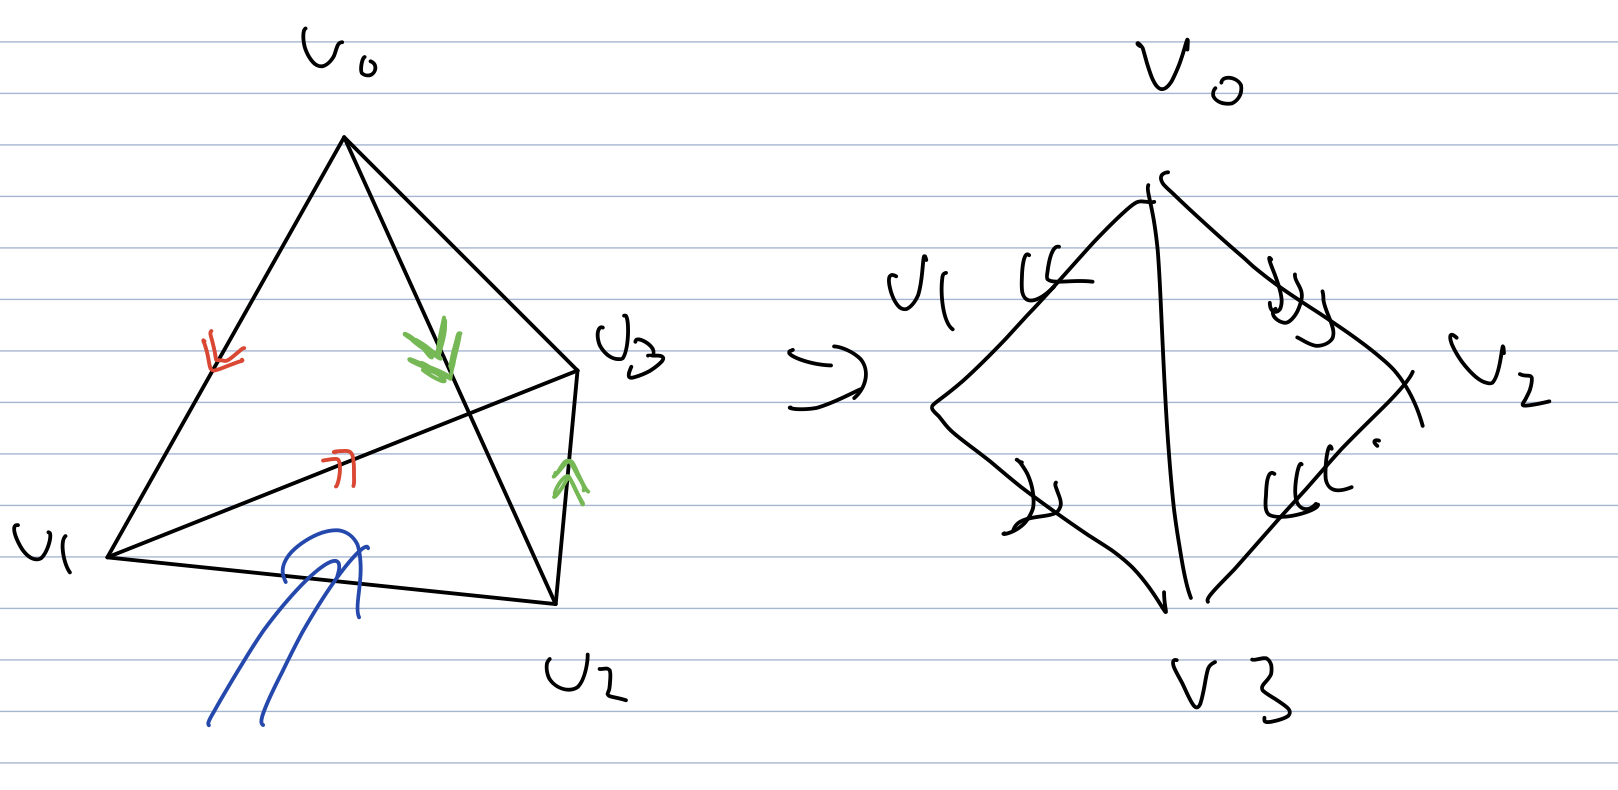
\includegraphics[width=.5\linewidth]{klein_delta3.jpeg}
  \caption{mycaption}
  \label{fig:mylabel}
  \end{figure}
\end{proof}

\begin{exer}{(Problem 4)}
  Compute the simplicial homology groups of the triangular parachute obtained from $\Delta^2$ by identifying its three vertices to a single point.
\end{exer}

\begin{proof}
  \todo[inline,caption={}]{
    Do I need to do the ``no-edge-can-have-the-same-vertices" thing?
  }
\end{proof}

\end{document}


